\chapter{Appendices}
\label{cha:appendices}

\section{AlloPred documentation}

This section contains documentation for the AlloPred source code, which can be found at \url{https://github.com/jgreener64/allopred}.


\subsection{Requirements}

\begin{itemize}
\item Python 2.7 with the NumPy and ProDy packages installed.
\item fpocket v2.0, which can be downloaded from \url{http://fpocket.sourceforge.net}. Follow the installation instructions to compile the executables.
\item SVM-light, which can be downloaded from \url{http://svmlight.joachims.org}. Follow the installation instructions to compile the executables.
\end{itemize}


\subsection{Usage}

Follow these steps to set up AlloPred - the shell commands are for bash:

\begin{enumerate}
\item Download the files and extract them as usual, or clone the repository.
\item The environmental variables \verb|$ALLOPRED_DIR| and \verb|$SVM_LIGHT_DIR| need to be set as the filepaths to the AlloPred directory and the SVM-light directory respectively:
\begin{lstlisting}[language=bash]
    export ALLOPRED_DIR=/path/to/allopred/
    export SVM_LIGHT_DIR=/path/to/svm_light/
\end{lstlisting}
Consider adding these lines to your profile so you don't have to run them every session.
\end{enumerate}

Follow these step to run AlloPred:

\begin{enumerate}
\item Obtain a PDB format file (\verb|in_file.pdb|), e.g.\ from the Protein Data Bank.

\item Create a one-line file (\verb|act_res.txt|) containing the active site residues of the protein. The format is \verb|10:A,11:B| for residue 10 on chain A and residue 11 on chain B. These can be found using resources such as the Catalytic Site Atlas. An example PDB file and active residue file can be found in the example directory of AlloPred.

\item Run fpocket v2.0 on the PDB file:
\begin{lstlisting}[language=bash]
    fpocket -f in_file.pdb
\end{lstlisting}
This assumes \verb|fpocket| is on the path. This produces the directory \verb|in_file_out|. AlloPred is optimised on the default fpocket parameters but you can change these in accordance with the fpocket documentation if you wish.

\item The following command, from the directory containing \verb|in_file.pdb| and \verb|in_file_out|, runs the AlloPred pipeline:
\begin{lstlisting}[language=bash]
    python $ALLOPRED_DIR/run_allopred.py in_file act_res.txt
\end{lstlisting}
The arguments are the input file prefix and the path to the active site residue file. Running the \verb|run_allopred.py| script with fewer than 2 arguments returns these instructions for the command.

\item The output files are:
    \begin{itemize}
    \item \verb|in_file.out|: the AlloPred output file containing the input parameters and the values for each pocket in order of AlloPred ranking.
    \item \verb|in_file.svm|: the SVM input file in the SVM-light format.
    \end{itemize}
\end{enumerate}


\subsection{Other files}

\begin{itemize}
\item \verb|dataset| contains information on the training and testing sets.
\item \verb|example| contains the inputs and outputs of an example run using the PDB entry with ID 1FX2.
\item \verb|svm_model.txt| is the optimised SVM built on the whole training set.
\end{itemize}


\section{ExProSE documentation}

This section contains documentation for the ExProSE source code, which can be found at \url{https://github.com/jgreener64/ProteinEnsembles.jl}.
% Version info


\subsection{Summary}

Install using \verb|Pkg.add("ProteinEnsembles")| from within Julia v0.5. Run using

\begin{lstlisting}[language=bash]
    exprose --i1 input_1.pdb --d1 input_1.dssp \
        --i2 input_2.pdb --d2 input_2.dssp \
        -n 50 -o exprose_out
\end{lstlisting}

where \verb|exprose| is in the \verb|bin| directory.


\subsection{Installation}

Julia v0.5 is required and can be downloaded from \url{http://julialang.org/downloads}. Install ProteinEnsembles.jl by running \verb|Pkg.add("ProteinEnsembles")| from the Julia REPL. This will also automatically install a few other required Julia packages. If you want, the tests can be run using \verb|Pkg.test("ProteinEnsembles")|. If you wish to use the auto-parameterisation procedure (see below) you must also have TM-score installed.


\subsection{Requirements}

To use ProteinEnsembles.jl you will need the following:
\begin{itemize}
\item PDB files of the protein of interest. Two is best, but one may be used (see the paper). They must have polar hydrogens only added; this can be done using tools such as Chimera or pdbtools. The chain labelling and residue numbering must be consistent between the files as this is used to find common atoms. Alternative atom locations are discarded. PDB files must also be a single model and not have any inserted residues. HETATM records are discarded by default.
\item DSSP files corresponding to the PDB files above. These can be obtained using dssp.
\end{itemize}


\subsection{Usage}

These instructions are tailored towards Mac/Unix. However they could be modified to work on Windows.

Although organised as a Julia package, ProteinEnsembles.jl is primarily designed for use from the command line. The \verb|exprose| script in the \verb|bin| directory implements this. For example, to see the command line options run

\begin{lstlisting}[language=bash]
    ~/.julia/v0.5/ProteinEnsembles/bin/exprose -h
\end{lstlisting}

For easy access to the \verb|exprose| command you might like to add the following line to your profile:

\begin{lstlisting}[language=bash]
    export PATH=$PATH:~/.julia/v0.5/ProteinEnsembles/bin
\end{lstlisting}

Then, if all input files are in your current directory, run the program as follows:

\begin{lstlisting}[language=bash]
    # Generate an ensemble of 50 structures with an output directory exprose_out
    exprose --i1 input_1.pdb --d1 input_1.dssp --i2 input_2.pdb \
        --d2 input_2.dssp -n 50 -o exprose_out

    # Use a tolerance weighting of 0.5
    exprose --i1 input_1.pdb --d1 input_1.dssp --i2 input_2.pdb \
        --d2 input_2.dssp -n 50 -o exprose_out -w 0.5

    # Generate an ensemble from a single structure with a tolerance weighting of 1.0
    exprose --i1 input_1.pdb --d1 input_1.dssp -n 50 -o exprose_out -w 1.0
\end{lstlisting}

The method may also be run from within Julia. The below Julia script does the same thing as the first example above:

\begin{lstlisting}
    using ProteinEnsembles
    runpipeline(
        i1="input_1.pdb",
        d1="input_1.dssp",
        i2="input_2.pdb",
        d2="input_2.dssp",
        n_strucs=50,
        out_dir="exprose_out"
    )
\end{lstlisting}

Or, to split it up a little into the constituent functions:

\begin{lstlisting}
    using ProteinEnsembles
    constraints_com, constraints_one, constraints_two = interactions(
        "input_1.pdb",
        "input_1.dssp",
        "input_2.pdb",
        "input_2.dssp"
    )
    ensemble_com = generateensemble(constraints_com, 50)
    runanalysis("exprose_out", ensemble_com, constraints_one, constraints_two)
\end{lstlisting}


\subsubsection{Selecting parameters}

The auto-parameterisation procedure can select a more suitable tolerance weighting value (see the paper). TM-score must be installed to do this. For example:

\begin{lstlisting}[language=bash]
    exprose-param --i1 input_1.pdb --d1 input_1.dssp --i2 input_2.pdb \
        --d2 input_2.dssp -o exprose_param -t TMscore
\end{lstlisting}

runs the auto-parameterisation procedure with the \verb|-t| option specifying the command to run TM-score. The last line of the output gives a suggested tolerance weighting. This value is also written out to \verb|suggested.tsv|. Use this value in a normal \verb|exprose| run as above.


\subsubsection{Allosteric site prediction}

To predict allosteric sites you should run LIGSITE\textsuperscript{\it cs} on the \emph{second} input structure (the one you give as \verb|--i2|). You then need to run the \verb|cluster-ligsite| script in \verb|bin| to assign the points to pockets:

\begin{lstlisting}[language=bash]
    cluster-ligsite pocket_r.pdb pocket_all.pdb pocket_points.pdb
\end{lstlisting}

where \verb|pocket_r.pdb| and \verb|pocket_all.pdb| are in the LIGSITE\textsuperscript{\it cs} output. Then carry out an \verb|exprose| run with the \verb|pocket_points.pdb| file (\verb|-l|) and the number of pockets (e.g.\ top 4) to perturb at (\verb|-m|) as parameters:

\begin{lstlisting}[language=bash]
    exprose --i1 input_1.pdb --d1 input_1.dssp --i2 input_2.pdb \
        --d2 input_2.dssp -n 50 -o exprose_out -l pocket_points.pdb -m 4
\end{lstlisting}

A tolerance weighting from an auto-parameterisation run can also be used here. View the \verb|predictions.tsv| output file to get the order of allosteric pocket predictions. Note that other pocket prediction software can be used provided you can get the output into the same format as \verb|pocket_points.pdb|, i.e. pocket cavity points with the pocket number in the residue number column.


\subsubsection{Output}

The output directory contains the following:
\begin{itemize}
\item \verb|input_1.pdb| and \verb|input_2.pdb|: atoms used from the input structures are written back out and superimposed.
\item \verb|pdbs|: generated structures in PDB format. Superimposed to \verb|input_1.pdb| and \verb|input_2.pdb|.
\item \verb|pcs|: projections onto the principal components (PCs) from the principal component analysis of the generated structures. Contains files for generated (\verb|pcs.tsv|) and input structures (\verb|pcs_input_1.tsv| and \verb|pcs_input_2.tsv|) - line n corresponds to structure n and column c corresponds to PC c. Has graphs of these for the first few PCs (\verb|pc_x_y.png|). Also includes a list of PCs ordered by decreasing distance betwen the input structures (\verb|pcs_input_dist.tsv|) and the percentage variation explained by each PC (\verb|evals_spread.tsv|).
\item \verb|pymol|: PyMol scripts to view PCs on \verb|input_1.pdb|, e.g.\ run \verb|pymol input_1.pdb pymol/view_pc_1.pml|.
\item \verb|rmsds_input_1.tsv| and \verb|rmsds_input_2.tsv|: RMSDs of generated structures to the input structures. Line n corresponds to structure n.
\item \verb|rmsfs.tsv| and \verb|rmsfs.png|: RMSFs of each residue over the ensemble of generated structures, and a plot of this. Line n corresponds to residue index n.
\item \verb|spe_scores.tsv|: SPE error scores of generated structures (see paper). Line n corresponds to structure n.
\end{itemize}

For allosteric site prediction there will be \verb|pdbs_mod_n| and \verb|mod_n| containing similar information for each perturbed ensemble, as well as the ratio of RMSF values to the unperturbed ensemble (\verb|rmsfs_ratio.tsv|). There will also be the order of allosteric predictions (\verb|predictions.tsv|) and the size of the perturbation on modulating each site (\verb|perturbations.tsv|), which is the RMSD between the centroid structure of the perturbed and unperturbed ensembles.

The default plot colours are blue for generated structures, red for input structure 1, green for input structure 2 and orange for perturbed ensemble structures.


\section{BioJulia Bio.Structure module}

The structure of the type heirarchy is based on Biopython \cite{Cock2009} and is shown in Figure~\ref{fig:model_structure}.
Examples of basic use cases for Bio.Structure are shown in Figure~\ref{fig:biojulia_example}.


\begin{figure}
\centering

\includegraphics[width=0.9\textwidth]{figures/model_structure/model_structure}

\caption{Type structure of the BioJulia Bio.Structure module.
Types, analogous to classes in other languages, are shown in text.
\texttt{StructuralElement}, \texttt{AbstractResidue} and \texttt{AbstractAtom} are abstract types and may not themselves be instantiated.
Concrete (i.e.\ not abstract) types are shown in bold text.
Subtypes, analogous to subclasses, are indicated by red dotted lines.
A blue line indicates that an instance of the type contains a list of the indicated type.
For example, a \texttt{Chain} contains multiple \texttt{AbstractResidue}s.}

\label{fig:model_structure}
\end{figure}


\begin{figure}
\centering

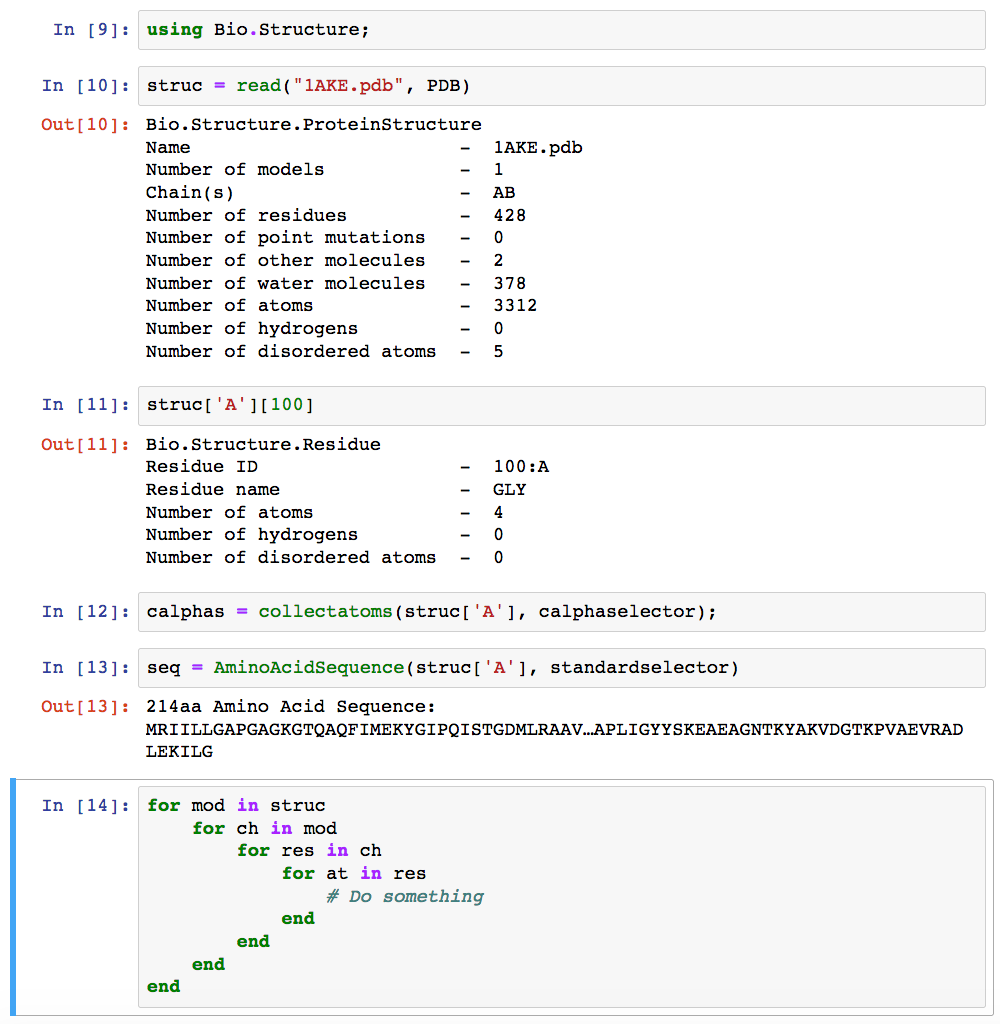
\includegraphics[width=0.9\textwidth]{figures/biojulia_example/biojulia_example}

\caption{Example functionality of the Bio.Structure module.
The Jupyter Notebook and Julia v0.5.2 are used.
Cases shown are importing the module, reading in a PDB file, accessing residues by index, extracting C\textsuperscript{\textalpha} atoms, extracting the amino acid sequence and iterating over sub-elements.}
% cite Jupyter? Possibly http://ebooks.iospress.nl/publication/42900

\label{fig:biojulia_example}
\end{figure}
